\part{Exercice 23}

\begin{enumerate}
	\item[5. ] Soit $f: x \mapsto \frac{1}{2+x}$.\\
		$f$ est dérivable sur $\R\setminus \{2\}$ et décroissante sur $]-\infty;2[$ et sur $]2;+\infty[$.\\
		\begin{center}
			\begin{tikzpicture}
				\tkzTabInit{$x$/1,  $f$/2}{$-\infty$,$-2$,$+\infty$}
				\tkzTabVar{+/$0$,-D+/$-\infty$/$+\infty$,-/ $0$}
			\end{tikzpicture}
		\end{center}
		On pose $g: x \mapsto f(x)- x = \frac{1}{2 +x} - x$ dérivable sur $\R\setminus \{2\}$ et \[
		\forall x \neq 2, g'(x) = -\frac{1}{(2+x)^2} -1 < 0
		\] 
		\begin{center}
			\begin{tikzpicture}
				\tkzTabInit{$x$/1,  $g$/2}{$-\infty$,$-2$,$+\infty$}
				\tkzTabVar{+/$-\infty$,-D+/$-\infty$/$+\infty$,-/ $-\infty$}
				\tkzTabVal12{0.5}{$\alpha$}0
				\tkzTabVal23{0.5}{$\beta$}0
			\end{tikzpicture}\\
			\begin{tikzpicture}
				\tkzTabInit{$x$/1,  $f$/2, $f(x)-x$/2}{$-\infty$,$\alpha$,$-2$,$\beta$,$+\infty$}
				\tkzTabVar{+/$0$,R,-D+/$-\infty$/$+\infty$,R,-/ $0$}
				\tkzTabVal13{0.5}{$\alpha$}{$\alpha$}
				\tkzTabVal35{0.5}{$\beta$}{$\beta$}
				\tkzTabLine{,+,z,-,d,+,z,-}
			\end{tikzpicture}
		\end{center}

		$(u_n)$ n'est pas définie s'il existe $k \in \N$ tel que \[
		f^k(u_0) = -2
		\] ($f^k(x) \neq (f(x))^k$, $f^k = f \circ \cdots \circ f$)

		\begin{itemize}
			\item On suppose la suite bien définie, 
				\begin{align*}
					\forall x \neq -2, \left| f'(x) \right| &= \left| -\frac{1}{(2+x)^2} \right|\\
																									&= \frac{1}{(2+x)^2}
				\end{align*}
				En particulier si $x>0$, alors $f'(x) \le \frac{1}{4}$ 
			\item On suppose $u_0 > -2$ alors $u_1 >0$ et donc \[
				\forall  n \in  \N_*, u_n > 0
				\] Donc \[
				\forall  n \in \N_*, \left| u_{n+1} - \beta \right| = \left| f(u_n) - f(\beta) \right| \le \frac{1}{4} \left| u_n - \beta \right| 
				\] On en déduit par récurrence que \[
				\forall n \in \N_*, \left| u_n- \beta \right| \le \left( \frac{1}{4} \right) ^{n-1} \left| u_1 - \beta \right| 
				\] Or, $\left( \frac{1}{4} \right)^{n-1} \tendsto{n \to +\infty} 0$\\
				Donc, $u_n \tendsto{n \to  +\infty} \beta$
			\item Si $u_0 = \alpha$ alors \[
					\forall n \in \N, u_n = \alpha \tendsto{n \to +\infty} \alpha
				\] 
			\item Si, $u_0 < -2$ et $u_0 \neq \alpha$, je conjecture qu'il existe $p \in \N_*$ tel que $u_p > -2$ et alors $u_n \tendsto{n \to +\infty} \beta$
		\end{itemize}
\end{enumerate}
